% (The MIT License)
%
% Copyright (c) 2023 Yegor Bugayenko
%
% Permission is hereby granted, free of charge, to any person obtaining a copy
% of this software and associated documentation files (the 'Software'), to deal
% in the Software without restriction, including without limitation the rights
% to use, copy, modify, merge, publish, distribute, sublicense, and/or sell
% copies of the Software, and to permit persons to whom the Software is
% furnished to do so, subject to the following conditions:
%
% The above copyright notice and this permission notice shall be included in all
% copies or substantial portions of the Software.
%
% THE SOFTWARE IS PROVIDED 'AS IS', WITHOUT WARRANTY OF ANY KIND, EXPRESS OR
% IMPLIED, INCLUDING BUT NOT LIMITED TO THE WARRANTIES OF MERCHANTABILITY,
% FITNESS FOR A PARTICULAR PURPOSE AND NONINFRINGEMENT. IN NO EVENT SHALL THE
% AUTHORS OR COPYRIGHT HOLDERS BE LIABLE FOR ANY CLAIM, DAMAGES OR OTHER
% LIABILITY, WHETHER IN AN ACTION OF CONTRACT, TORT OR OTHERWISE, ARISING FROM,
% OUT OF OR IN CONNECTION WITH THE SOFTWARE OR THE USE OR OTHER DEALINGS IN THE
% SOFTWARE.

\documentclass{article}
\usepackage{../pmba}
\newcommand*\thetitle{Risk Management}
\begin{document}

\plush{\pmbaTitlePage{8}}

% reserves: management reserve too, contingency reserve

\plush{
\pptBanner{Management \st{Triangle} Rectangle}\par
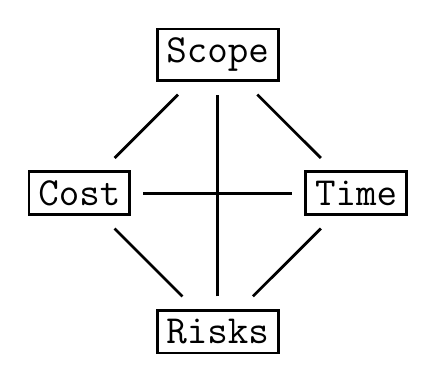
\begin{tikzpicture}[node distance=5em,
  every path/.style={draw=black, line width=.1em},
  every node/.style={font={\Large\ttfamily}, draw=black, rectangle, outer sep=.5em}]
\node[draw=none] (center) {};
\node[above of=center] (scope) {Scope};
\node[below of=center] (risks) {Risks};
\node[right of=center] (time) {Time};
\node[left of=center] (cost) {Cost};
\path (scope) -- (time);
\path (time) -- (cost);
\path (cost) -- (scope);
\path (risks) -- (time);
\path (risks) -- (cost);
\path (risks) -- (scope);
\end{tikzpicture}
}

\pmbaQuestion
  {You just found out that one of your key programmers posted his resume on a job board. What do you do immediately?}
  {Update risk list}
  {Post a vacation}
  {Offer him a raise}
  {Nothing}
  {staff}

\pmbaQuestion
  {What is the cost of a risk, if \emph{probablity} is 0.8, \emph{impact} is 0.7, and \emph{effect} is \pounds1,000?}
  {\pounds1,500}
  {\pounds560}
  {\pounds800}
  {\pounds700}
  {quantitative}

\pmbaQuestion
  {What is the name of a risk with a \emph{negative value} of the \emph{impact}?}
  {Opportunity}
  {Residual Risk}
  {Threat}
  {?}
  {register}

\pmbaQuestion
  {What is the relation of elements in the cause-risk-effect format?}
  {Many-one-many}
  {Many-many-many}
  {Many-one-one}
  {One-one-one}
  {format}

\pmbaQuestion
  {There is a \emph{risk} that the server will break. If this happens, a new one will cost another \$5,000. How to prepare the customer for this?}
  {Ask him to pay \$5K upfront, refund later}
  {Put \$5K into contingency reserve}
  {Put \$5K into management reserve}
  {Put \$2.5K into project budget}
  {reserves}

\plush{
  \pptBanner{Homework:}
  ``\emph{Risk Register} is a document in which the results of risk analysis and risk response planning
  are recorded. It contains the outcomes of the other risk management processes as they are
  conducted, resulting in an increase in the level and type of information contained in the
  risk register over time.'' --- PMBOK5
}

\plush{
  \pptBanner{Read this:}
  Risk Management by Rita Mulcahy\par
  \href{}{} ()\par
  \href{}{} ()\par
  \href{}{} ()\par
  \href{}{} ()\par
  \href{}{} ()\par
  \href{}{} ()\par
  \href{}{} ()\par
}

\end{document}
